\documentclass[Doctor]{BJTU-thesis}

%%%%%%%%%%%%%%%%%%%引入一些包%%%%%%%%%%%%%%%%%%%%%
\usepackage{emptypage}

% 字体
\setromanfont{Times New Roman}
\usepackage{fontspec}
\newfontfamily\myfont{times.ttf}
\setmainfont{Times New Roman}
\renewcommand\labelenumi{(\theenumi)}

% 标题相关
\usepackage{bicaption}
\captionsetup[figure][bi-first]{name=图}
\captionsetup[figure][bi-second]{name=Figure}
\captionsetup[table][bi-first]{name=表}
\captionsetup[table][bi-second]{name=Table}

% 算法相关
\usepackage[ruled,linesnumbered,algochapter]{algorithm2e}
\renewcommand{\algorithmcfname}{算法}
\SetKwInput{KwIn}{输入}
% \SetKwData{KwData}{输入}
\SetKwInOut{Return}{返回}
\SetAlgoNoLine
% 将编号改为chapter-number
\makeatletter
\renewcommand\thealgocf{\csname the\algocf@within\endcsname-\@arabic\c@algocf}
\makeatother

% 表格
\usepackage{pifont} % 表格
\usepackage{diagbox} % 表格
\usepackage{booktabs}
\usepackage{chngpage}

% 图片
\graphicspath{{./figure/}} % 图片

%%%%%%%%%%%%%%%填写封面信息%%%%%%%%%%%%%%%%%%%%
\author{曹旭阳}
\studentNumber{17111058}
\advisor{陈后金}
\advisorTitle{教授}
 
\degreeType{工学}
\major{电子科学与技术}
\researchArea{图像处理与模式识别}
\title{基于深度学习的三维自动乳腺超声图像分割方法研究}
\englishtitle{Research on Deep Learning Based 3D Automatic Breast Ultrasound Image Segmentation}

% \makeindex
\makeindex[name=class,options=-s mystyle,title=分类索引,columns=2]
\makeindex[name=author,options=-s mystyle,title=著者索引,columns=2]
\makeindex[name=keyword,options=-s mystyle,title=关键词索引,columns=2]

\begin{document}
\makecover
\makeAuthorization
\makeInfo

\thispagestyle{empty}{
\begin{thanks}

致谢

\end{thanks}
 }

\begin{abstract}

中文摘要内容

\vspace{16pt}
\noindent
\keywords{深度学习;乳腺ABUS图像;肿瘤分割;神经网络架构搜索;半监督学习}

\noindent
\classno{TP391}

\end{abstract}


%% English Abstract %%
\begin{englishabstract}

English Abstract

\vspace{16pt}
\noindent
\englishkeywords{Deep Learning; ABUS Image; Breast Tumor segmentation; Neural Architecture Search; Semi-Supervised Learning}

\noindent
\englishclassno{TP391}

\end{englishabstract}
% \begin{preface}
    \begin{tabbing}
        CNN      卷积神经网络 \\
    
        ROI      感兴趣区域 \\
    
    \end{tabbing}
\end{preface}
\tableofcontents

% 正文部分
\newpage\pagenumbering{arabic}
\chapter{绪论}

以下给出一些常用命令。

参考文献引用\cite{abdar_uncertainty_2021, baumgartner_exploration_2018, ackley_learning_1985}

\begin{equation}
    \label{equ:basic_chain_rule}
    \begin{split}
        \frac{\partial L}{\partial \boldsymbol{W_3}} &= \frac{\partial L}{\partial f_3} \cdot \frac{\partial f_3}{\partial \boldsymbol{W_3}} \\
        \frac{\partial L}{\partial \boldsymbol{W_2}} &= \frac{\partial L}{\partial f_3} \cdot \frac{\partial f_3}{\partial f_2} \cdot \frac{\partial f_2}{\partial \boldsymbol{W_2}}  \\
        \frac{\partial L}{\partial \boldsymbol{W_1}} &= \frac{\partial L}{\partial f_3} \cdot \frac{\partial f_3}{\partial f_2} \cdot \frac{\partial f_2}{\partial f_1} \cdot \frac{\partial f_1}{\partial \boldsymbol{W_1}} \\
    \end{split}
\end{equation}

\begin{algorithm}[!ht]
    \caption{反向传播算法}
    \label{alg:basic_back_propagation}

    \KwIn{$l$层神经网络}
    \KwIn{激活函数$f_i \text{, } i\in l$}
    \KwIn{输出数据$\boldsymbol{x}$,真实标签$\boldsymbol{y}$}
    
    计算前向传播:$\boldsymbol{\hat{y}} = f_l \left( \boldsymbol{W_l} \ldots f_2 \left( \boldsymbol{W_2} f_1 \left( \boldsymbol{W_1 x} \right) \right) \right)$
    
    计算输出结果与真实标签之间误差:$L = loss \left( \boldsymbol{\hat{y}}, \boldsymbol{y} \right)$
    
    计算初始梯度:$\delta = \partial L / \partial f_{l}$

    \For{$i$ in $\left[ l, 0, -1 \right]$}
    {
        根据链式法计算损失函数关于第$i$层网络权重$\boldsymbol{W_i}$的偏导:$\partial L / \partial \boldsymbol{W_i} = \delta \cdot \partial f_i / \partial \boldsymbol{W_i}$
        
        使用优化算法对当前层网络权重进行更新,如梯度下降法
        
        将当前梯度反向传播至前一层:$\delta = \delta \cdot \partial f_i / \partial f_{i-1}$
    }
\end{algorithm}

\begin{figure}[!ht]
    \centering
    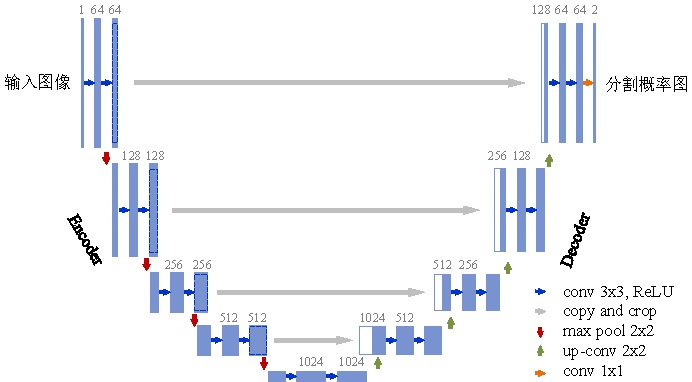
\includegraphics[width=0.9\textwidth]{figure/basic_theory/unet_arch}
    \bicaption{U-Net网络结构}{U-Net architecture}
    \label{fig:basic_unet_arch}
\end{figure}

\begin{figure}
     \centering
     \begin{subfigure}[t]{0.32\textwidth}
         \centering
         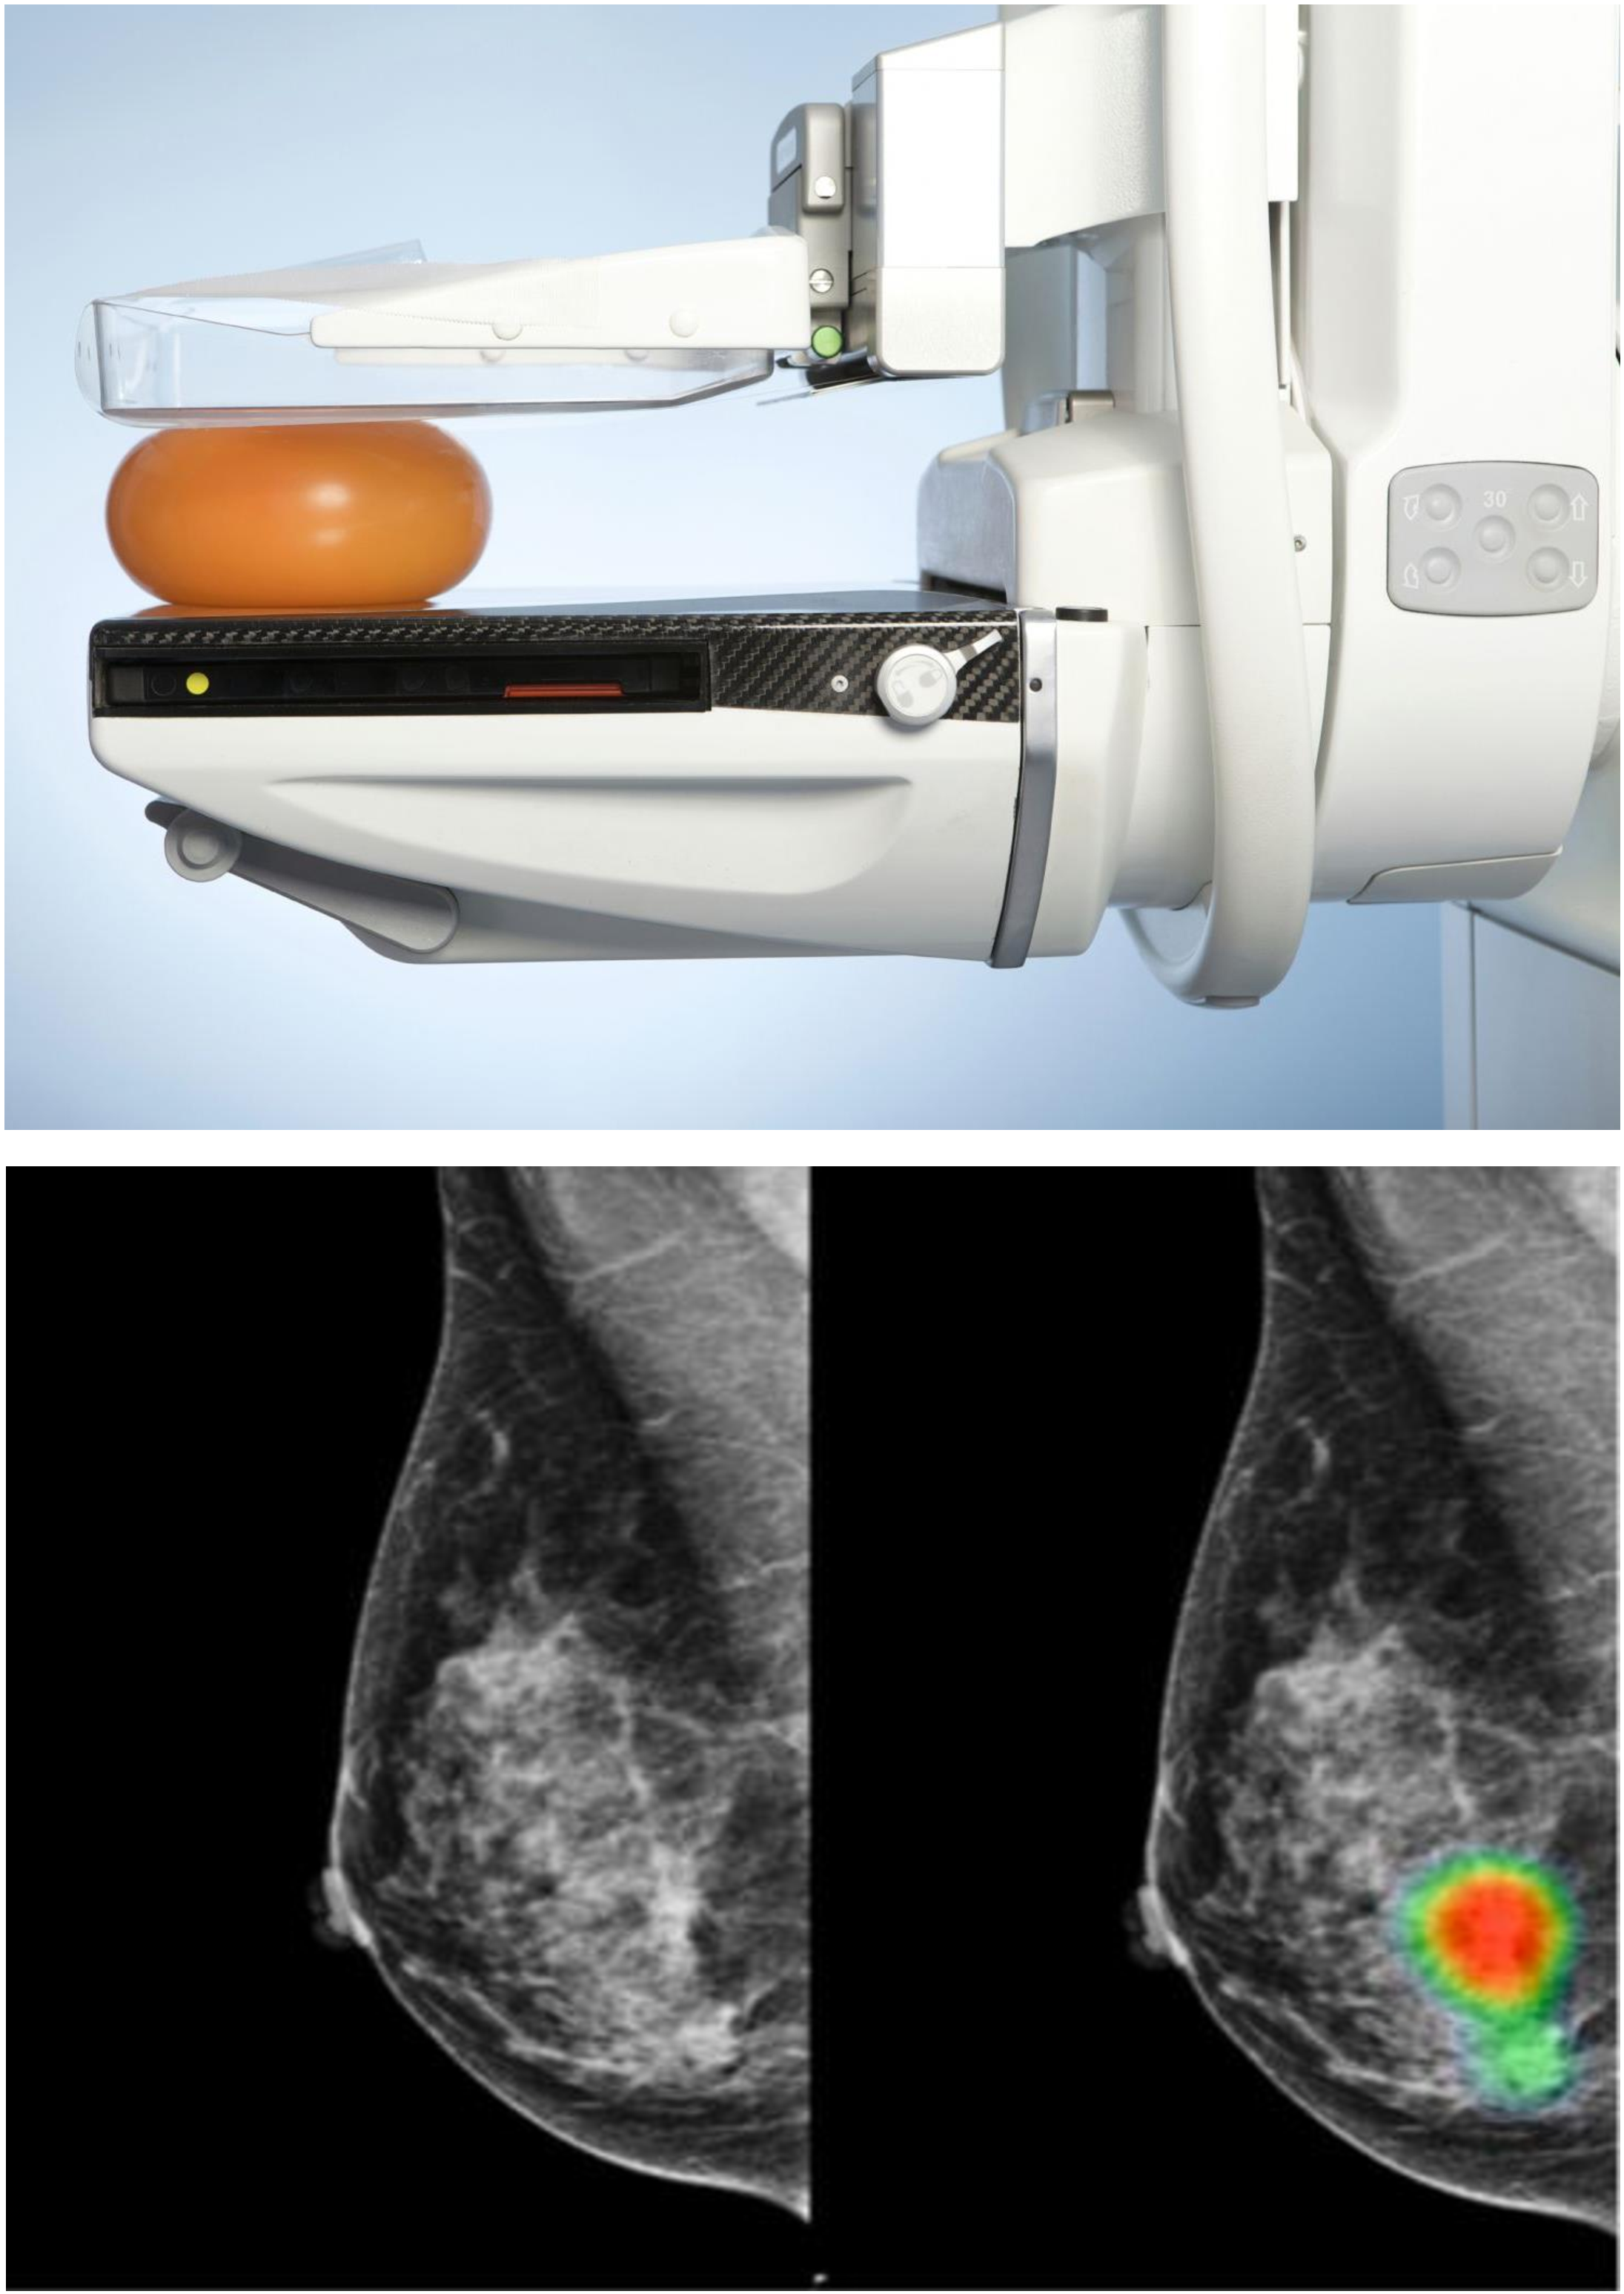
\includegraphics[width=\textwidth]{figure/introdution/mammogram}
         \bicaption{X线钼靶}{Mammography}
         \label{subfig:mammography}
     \end{subfigure}
     \begin{subfigure}[t]{0.32\textwidth}
         \centering
         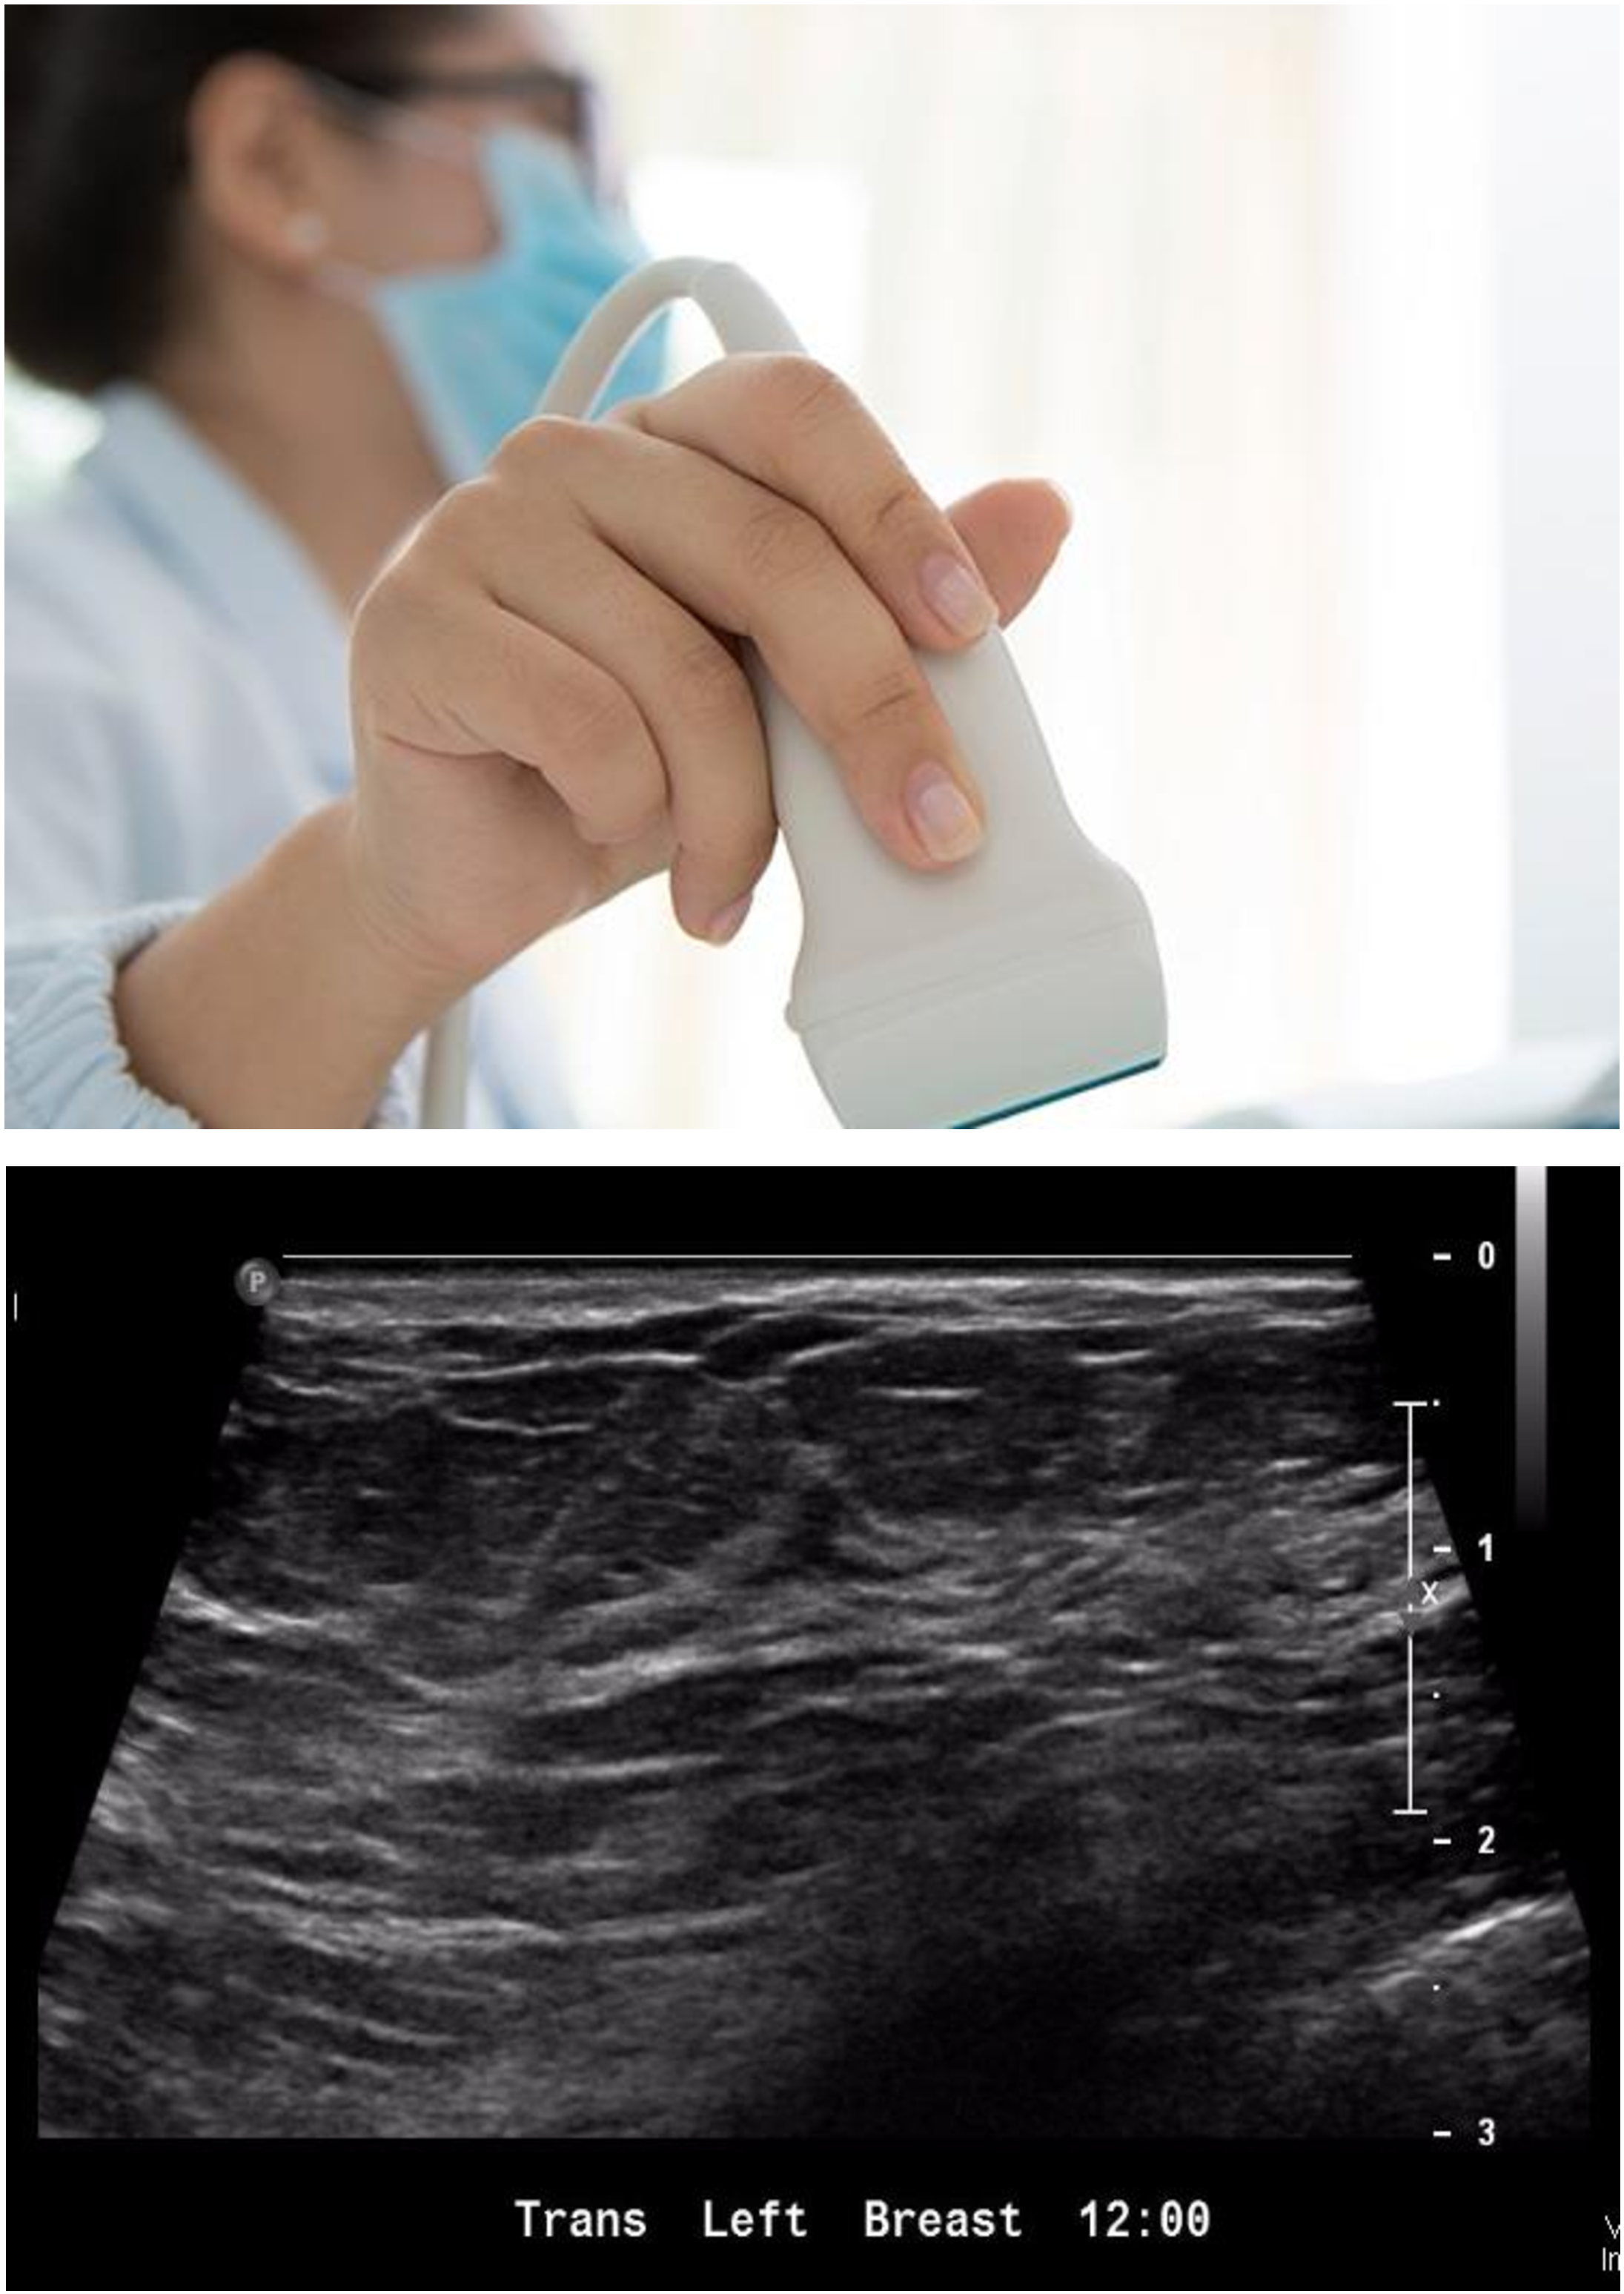
\includegraphics[width=\textwidth]{figure/introdution/bus}
         \bicaption{手动乳腺超声}{Handheld breast ultrasound}
         \label{subfig:bus}
     \end{subfigure}
     \begin{subfigure}[t]{0.32\textwidth}
         \centering
         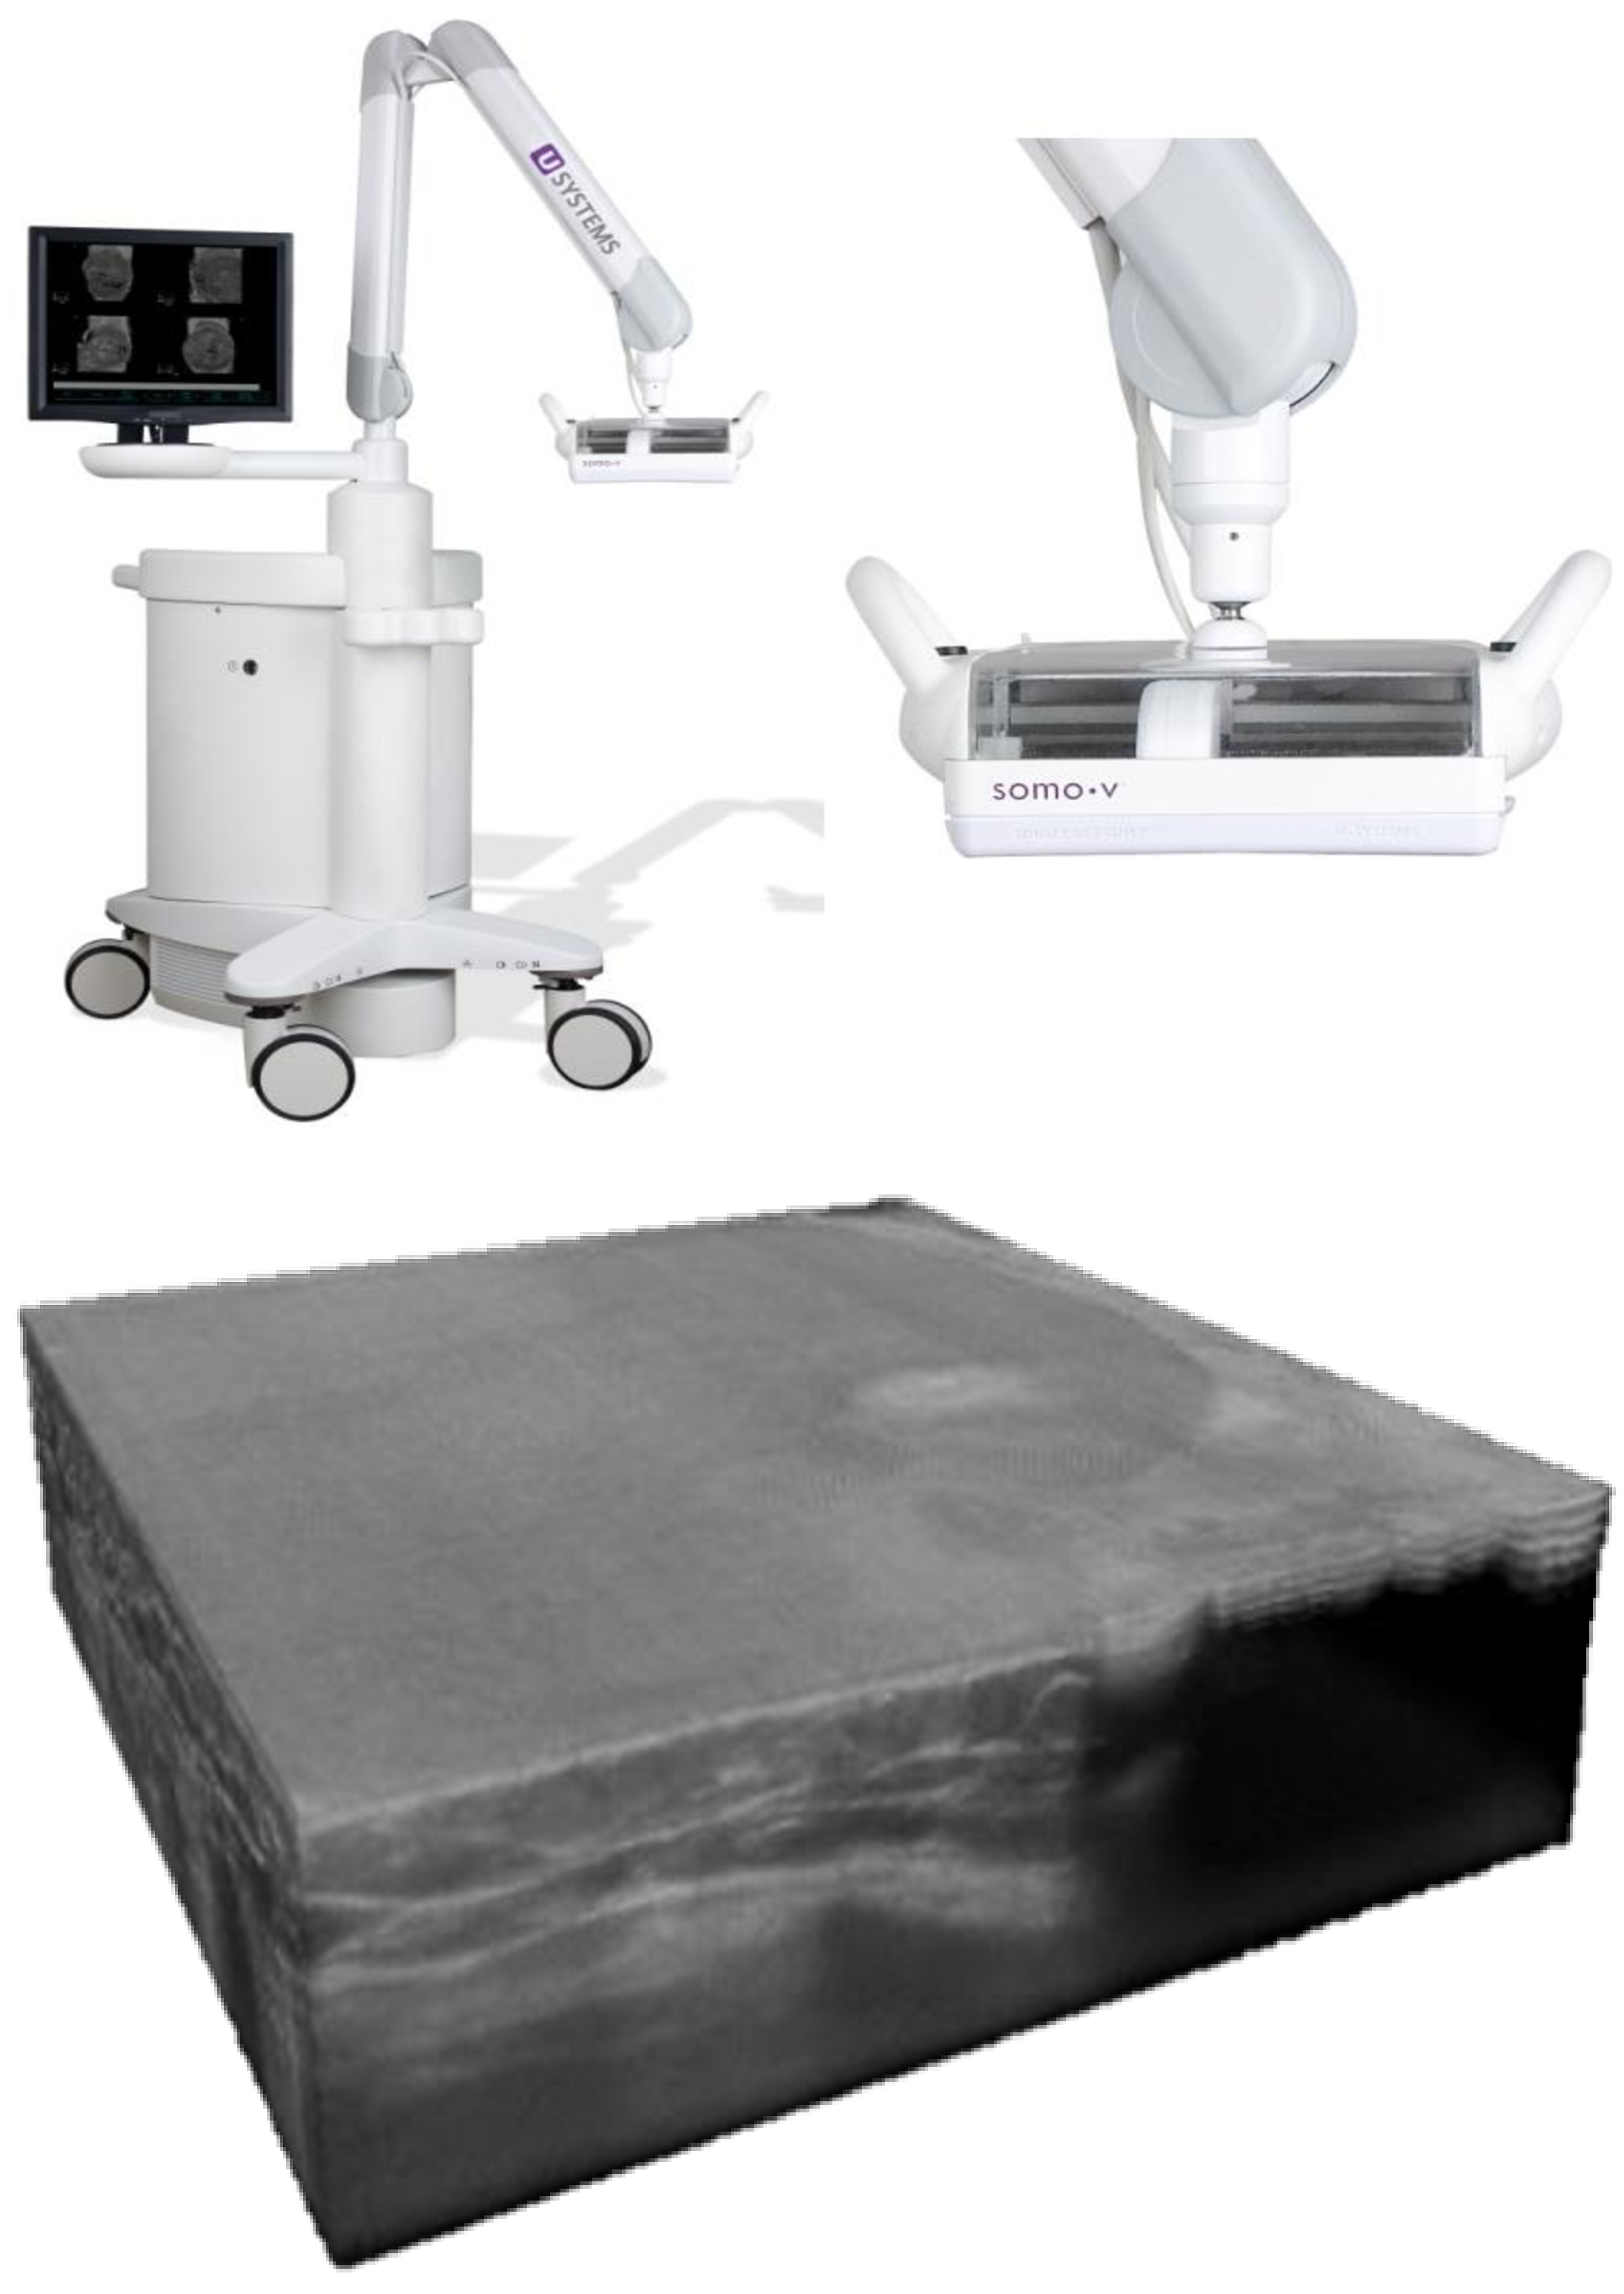
\includegraphics[width=\textwidth]{figure/introdution/abus}
         \bicaption{乳腺自动超声}{Automated breast ultrasound}
         \label{subfig:abus}
     \end{subfigure}
    \bicaption{不同乳腺成像仪器及对应的影像模态}{Different breast imaging scanners and the corresponding imaging modalities}
    \label{fig:intro_diff_imaging_modalities}
\end{figure}

\begin{table}[!ht]
    \bicaption{使用不同数量有标签图像的全监督与半监督分割结果对比}{Quantitative segmentation results of supervised and semi-supervised methods under different numbers of labeled images}
    \centering
    \begin{tabular}{cccccc}
        \toprule
        有标签数量 / 无标签数量 & 方法 & JI &  DSC & Acc & HD \\
        \hline
        100 / 0 & 全监督 & 0.4695 & 0.5871 & 0.9827 & 14.30mm \\
        100 / 8756 & UATE & \textbf{0.5643} & \textbf{0.6727} & \textbf{0.9895} & \textbf{5.95mm}\\
        \hline
        300 / 0 & 全监督 & 0.5407 & 0.6552 & 0.9881 &  9.14mm\\
        300 / 8556 & UATE & \textbf{0.6215} & \textbf{0.7287} & \textbf{0.9910} & \textbf{4.39mm}\\
        \hline
        885 / 0 & 全监督 & 0.5756 & 0.6890 & 0.9897 & 8.06mm\\
        885 / 7971 & UATE & \textbf{0.6270} & \textbf{0.7328} & \textbf{0.9911} & \textbf{4.13mm}\\
        \hline
        1770 / 0 & 全监督 & 0.5933 & 0.7070 & 0.9904 & 7.06mm\\
        1770 / 7086 & UATE & \textbf{0.6316} & \textbf{0.7372} & \textbf{0.9912} & \textbf{3.92mm}\\
        \hline
        4428 / 0 & 全监督 & 0.5961 & 0.7089 & 0.9904 & 8.46mm\\
        4428 / 4428 & UATE & \textbf{0.6365} & \textbf{0.7425} & \textbf{0.9921} & \textbf{3.81mm}\\
        \hline
        8856 / 0 & 全监督 & 0.6078 & 0.7125 & 0.9911 & 5.34mm\\
        \bottomrule
    \end{tabular}
    \label{tab:uate_result_diff_sample_data}
\end{table}

\begin{table}[!ht]
    \centering
    \bicaption{Dense U-Net 网络结构}{Dense U-Net architectures}
    \begin{tiny}
    \begin{tabular}{c|c|c|c|c}
        \toprule
        Layers & Output Size & Dense U-Net 121 & Dense U-Net 161 & Dense U-Net 201 \\
        \hline
        Input Layer & $128\times 512$ & \multicolumn{3}{c}{-}\\
        \hline
        Convolution & $64\times 256$ & \multicolumn{3}{c}{$7\times 7$ conv, stride 2} \\
        \hline
        Pooling & $32 \times 128$ & \multicolumn{3}{c}{$3\times 3$ max pool, stride 2} \\
        \hline
        Dense Block 1 & $32\times 128$ & $\begin{bmatrix}1\times 1 \text{ conv} \\3\times 3 \text{ conv} \end{bmatrix}\times 6$ & $\begin{bmatrix}1\times 1 \text{ conv} \\3\times 3 \text{ conv} \end{bmatrix}\times 6$ & $\begin{bmatrix}1\times 1 \text{ conv} \\3\times 3 \text{ conv} \end{bmatrix}\times 6$\\ 
        \hline
        \multirow{2}{*}{Transition Layer 1} & $32\times 128$ & \multicolumn{3}{c}{$1\times 1$ conv} \\
        \cline{2-5}
         & $16\times 64$ & \multicolumn{3}{c}{$2\times 2$ average pool, stride 2} \\
        \hline
        Dense Block 2 & $16\times 64$ & $\begin{bmatrix}1\times 1 \text{ conv} \\3\times 3 \text{ conv} \end{bmatrix}\times 12$ & $\begin{bmatrix}1\times 1 \text{ conv} \\3\times 3 \text{ conv} \end{bmatrix}\times 12$ & $\begin{bmatrix}1\times 1 \text{ conv} \\3\times 3 \text{ conv} \end{bmatrix}\times 12$ \\
        \hline
        \multirow{2}{*}{Transition Layer 2} & $16\times 64$ & \multicolumn{3}{c}{$1\times 1$ conv} \\
        \cline{2-5}
         & $8\times 32$ & \multicolumn{3}{c}{$2\times 2$ average pool, stride 2} \\
        \hline
        Dense Block 3 & $8\times 32$ & $\begin{bmatrix}1\times 1 \text{ conv} \\3\times 3 \text{ conv} \end{bmatrix}\times 24$ & $\begin{bmatrix}1\times 1 \text{ conv} \\3\times 3 \text{ conv} \end{bmatrix}\times 36$ & $\begin{bmatrix}1\times 1 \text{ conv} \\3\times 3 \text{ conv} \end{bmatrix}\times 48$ \\
        \hline
        \multirow{2}{*}{Transition Layer 3} & $8\times 32$ & \multicolumn{3}{c}{$1\times 1$ conv} \\
        \cline{2-5}
         & $4\times 16$ & \multicolumn{3}{c}{$2\times 2$ average pool, stride 2} \\
        \hline
        Dense Block 4 & $4\times 16$ & $\begin{bmatrix}1\times 1 \text{ conv} \\3\times 3 \text{ conv} \end{bmatrix}\times 16$ & $\begin{bmatrix}1\times 1 \text{ conv} \\3\times 3 \text{ conv} \end{bmatrix}\times 24$ & $\begin{bmatrix}1\times 1 \text{ conv} \\3\times 3 \text{ conv} \end{bmatrix}\times 32$ \\
        \hline
        Up-Sampling Layer 1 & $8\times 32$ & $2\times 2$ upsampling, conv, 512 & $2\times 2$ upsampling, conv, 768 & $2\times 2 $ upsampling, conv, 512 \\
        \hline
        Up-Sampling Layer 2 & $16\times 64$ & $2\times 2$ upsampling, conv, 256 & $2\times 2$ upsampling, conv, 384 & $2\times 2$ upsampling, conv, 256 \\
        \hline
        Up-Sampling Layer 3 & $32\times 128$ & \multicolumn{3}{c}{$2\times 2$ upsampling, conv, 96} \\
        \hline
        Up-Sampling Layer 4 & $64\times 256$ & \multicolumn{3}{c}{$2\times 2$ upsampling, conv, 96} \\
        \hline
        Up-Sampling Layer 5 & $128\times 512$ & \multicolumn{3}{c}{$2\times 2$ upsampling, conv, 64} \\
        \hline
        Output Layer & $128\times 512$ & \multicolumn{3}{c}{$1\times 1$ conv, 2} \\
        \bottomrule
    \end{tabular}
    \end{tiny}
    \label{tab:uate_denseunet_architecture}
\end{table}
\chapter{一级标题}

\section{二级标题}

\subsection{三级标题}

\subsection{三级标题}

\subsection{三级标题}

\section{二级标题}

\subsection{三级标题}

\subsection{三级标题}

\subsection{三级标题}
\chapter{第三章} \label{cht:d2unet}

\section{二级标题}

\subsection{三级标题}

\subsection{三级标题}

\subsection{三级标题}

\section{二级标题}

\subsection{三级标题}

\subsection{三级标题}

\subsection{三级标题}
\chapter{第四章} \label{cht:boundary_loss}

\section{二级标题}

\subsection{三级标题}

\subsection{三级标题}

\subsection{三级标题}

\section{二级标题}

\subsection{三级标题}

\subsection{三级标题}

\subsection{三级标题}
\chapter{第五章} \label{cht:nas}

\section{二级标题}

\subsection{三级标题}

\subsection{三级标题}

\subsection{三级标题}

\section{二级标题}

\subsection{三级标题}

\subsection{三级标题}

\subsection{三级标题}
\chapter{第六章}

\section{二级标题}

\subsection{三级标题}

\subsection{三级标题}

\subsection{三级标题}

\section{二级标题}

\subsection{三级标题}

\subsection{三级标题}

\subsection{三级标题}
\chapter{总结与展望}
\bibliography{reference}
% 正文结束


% 附录
% \appendix
% \chapter[附录标题]{}
%	\addcontentsline{toc}{section}{附录\thechapter\hspace*{1em}附录标题}
\markboth{附录\thechapter}{}
\begin{center}
	\zihao{3}\bfseries 附录标题
\end{center}

[内容为五号宋体。] 附录是作为论文主体的补充项目,并不是必须的。
论文的附录依序用大写正体英文字母A、B、C……编序号,如:附录A。


%正文中加入index:
%This is my key\index{key}.
This is my second palace\index[class]{palace} that has a key.

上文提到Knuth留下了后门 \verb|\special|,但是直接用它来插入图形不够含蓄优雅,于是 \LaTeX v2.09 推出了\texttt{epsf} 和 \texttt{psfig} 宏包。之后David P. Carlisle (1961--) \index{著者索引!Carlisle@David P. Carlisle, 大卫·卡利斯}\footnote{1995年曼彻斯特大学\index[class]{edu.manchester@University of Manchester, 曼彻斯特大学}数学博士,剑桥博士后,1998年加入数字算法公司 (Numerical Algorithms Group) \index[author]{com.nag@Numerical Algorithms Group, 数字算法公司}。} 和Rahtz推出了面向 \LaTeXe 的 \texttt{graphics} 和 \texttt{graphicx} 宏包;后者基于前者,语法更简单,功能更强大,所以一般推荐用它。


\index{classfication!plus}

%% 索引
% \chapter*{索引}
% \pagestyle{fancy}
% \addcontentsline{toc}{chapter}{索引}
% 678
% \printindex[class]
% \addcontentsline{toc}{section}{分类索引}
% 456
% \printindex[author]
% \addcontentsline{toc}{section}{著者索引}
% 345
% \printindex[keyword]
% \addcontentsline{toc}{section}{关键词索引}
% 123

	\chapter*{作者简历及攻读博士学位期间取得的研究成果}
	\markboth{作者简历及攻读博士学位期间取得的研究成果}{}
\addcontentsline{toc}{chapter}{作者简历及攻读博士学位期间取得的研究成果}
%	[内容采用五号宋体]  包括教育经历、工作经历、攻读学位期间发表的论文和完成的工作等。行距16磅,段前后各为0磅。
	
一、作者简历

	\textbf{基本情况:}
	 

	\textbf{教育经历:}
	
 
	
	\textbf{研究兴趣:}
	 
	
	
二、发表论文
	\setlength\leftmargini{3.5em}
	\renewcommand\labelenumi{[\theenumi]}
	\begin{enumerate}
 	\item xxx
	\end{enumerate}

%	三、参与科研项目
%	\begin{enumerate}
%		\item e
%		\item yi
%		\item san
%	\end{enumerate}
%
%	四、专利
%	\begin{enumerate}
%		\item e
%		\item yi
%		\item san
%	\end{enumerate}
\chapter*{独创性声明}
\markboth{独创性声明}{}
\addcontentsline{toc}{chapter}{独创性声明}
本人声明所呈交的学位论文是本人在导师指导下进行的研究工作和取得的研究成果,除了文中特别加以标注和致谢之处外,论文中不包含其他人已经发表或撰写过的研究成果,也不包含为获得北京交通大学或其他教育机构的学位或证书而使用过的材料。与我一同工作的同志对本研究所做的任何贡献均已在论文中作了明确的说明并表示了谢意。

\vspace*{3em}
学位论文作者签名:\hfill 签字日期:\hspace*{4em}年\hspace*{2em}月\hspace*{2em}日
\chapter*{学位论文数据集}
\markboth{学位论文数据集}{}
\addcontentsline{toc}{chapter}{学位论文数据}
% Table generated by Excel2LaTeX from sheet 'Sheet1'
\hspace{-2em}
\begin{table}[!ht]
    \begin{adjustwidth}{-.4in}{-.4in}
	\centering
% 	\caption{数据集页}
	\begin{tabular}{|p{6.9em}llll|}
		\hline
		\multicolumn{1}{|p{6.9em}|}{关键词*} & \multicolumn{1}{p{6em}|}{密级*} & \multicolumn{1}{p{7em}|}{中图分类号} & \multicolumn{1}{p{8em}|}{UDC} & \multicolumn{1}{p{6em}|}{论文资助}\\
		\hline
		
		\multicolumn{1}{|p{6.9em}|}{深度学习;乳腺ABUS图像;肿瘤分割;神经网络架构搜索;半监督学习} & \multicolumn{1}{l|}{\multirow{5}{*}{公开}} & \multicolumn{1}{l|}{\multirow{5}{*}{TP391}} & \multicolumn{1}{l|}{} & \\
		\hline
		
		\multicolumn{2}{|p{12.9em}|}{学位授予单位名称*} & \multicolumn{1}{p{7em}|}{学位授予单位代码*} & \multicolumn{1}{p{8em}|}{学位类别*} & \multicolumn{1}{p{6em}|}{学位级别*} \\
		\hline
		
		\multicolumn{2}{|p{12.9em}|}{北京交通大学} & \multicolumn{1}{l|}{10004} & \multicolumn{1}{l|}{工学} &  博士\\
		\hline
		
		\multicolumn{2}{|p{12.9em}|}{论文题名*} & \multicolumn{2}{p{15em}|}{并列题名} & \multicolumn{1}{p{6em}|}{论文语种*} \\
		\hline
		
		\multicolumn{2}{|p{12.9em}|}{基于深度学习的三维自动乳腺超声图像分割方法研究} & \multicolumn{2}{l|}{} &  中文\\
		\hline
		
		\multicolumn{1}{|p{6.9em}|}{作者姓名*} & \multicolumn{2}{l|}{曹旭阳} & \multicolumn{1}{p{8em}|}{学号*} &  17111058 \\
		\hline
		
		\multicolumn{2}{|p{12.9em}|}{培养单位名称*} & \multicolumn{1}{p{7em}|}{培养单位代码*} & \multicolumn{1}{p{8em}|}{培养单位地址} & \multicolumn{1}{p{6em}|}{邮编} \\
		\hline
		
		\multicolumn{2}{|p{12.9em}|}{北京交通大学} & \multicolumn{1}{l|}{10004} & \multicolumn{1}{p{8em}|}{北京市海淀区西直门外上园村3号} & 100044 \\
		\hline
		
		\multicolumn{2}{|p{12.9em}|}{学科专业*} & \multicolumn{1}{p{7em}|}{研究方向*} & \multicolumn{1}{p{8em}|}{学制*} & \multicolumn{1}{p{6em}|}{学位授予年*} \\
		\hline
		
		\multicolumn{2}{|l|}{电路与系统} & \multicolumn{1}{p{7em}|}{图像处理与模式识别} & \multicolumn{1}{l|}{四年} & 2022 \\
		\hline
		
		\multicolumn{1}{|p{6.9em}|}{论文提交日期*} & \multicolumn{4}{r|}{} \\
		\hline
		
		\multicolumn{1}{|p{6.9em}|}{导师姓名*} & \multicolumn{2}{l|}{陈后金} & \multicolumn{1}{p{8em}|}{职称*} &  教授\\
		\hline
		
		\multicolumn{1}{|p{6.9em}|}{评阅人} & \multicolumn{2}{p{13em}|}{答辩委员会主席*} & \multicolumn{2}{p{14em}|}{答辩委员会成员} \\
		\hline
		
		\multicolumn{1}{|r|}{\multirow{2}[2]{*}{}} & \multicolumn{2}{r|}{\multirow{2}[2]{*}{}} & \multicolumn{2}{r|}{\multirow{2}[2]{*}{}} \\
		
		\multicolumn{1}{|r|}{} & \multicolumn{2}{r|}{} & \multicolumn{2}{r|}{} \\
		\hline
		
		\multicolumn{5}{|p{33.9em}|}{电子版论文提交格式  文本(~)  图像(~) 视频(~) 音频(~) 多媒体(~) 其他(~)} \\
		\multicolumn{5}{|p{33.9em}|}{推荐格式:application/msword;application/pdf} \\
		\hline
		
		\multicolumn{2}{|p{12.9em}|}{电子版论文出版(发布)者} & \multicolumn{2}{p{15em}|}{电子版论文出版(发布)地} & \multicolumn{1}{p{6em}|}{权限声明} \\
		\hline
		
		\multicolumn{2}{|r|}{} & \multicolumn{2}{r|}{} &  \\
		\hline
		
		\multicolumn{1}{|p{6.9em}|}{论文总页数*} & \multicolumn{4}{r|}{} \\
		\hline
		
		\multicolumn{5}{|p{33.9em}|}{共33项,其中带*为必填数据,为21项。} \\
		\hline
	\end{tabular}
	\end{adjustwidth}
	\label{tab:addlabel}
\end{table}

\end{document}